\documentclass[a4paper,11pt]{jsarticle}

% 数式
\usepackage{amsmath,amsfonts}
\usepackage{bm}
\usepackage{mathtools}

% 表
\usepackage[utf8]{inputenc}
\usepackage{diagbox}
\usepackage{booktabs}
\usepackage{hhline}

% 画像
\usepackage[dvipdfmx]{graphicx}
\usepackage{ascmac}
\usepackage{physics}
\usepackage{float}

% 図
\usepackage[dvipdfmx]{graphicx}
\usepackage{tikz}
\usetikzlibrary{positioning, intersections, calc, arrows.meta,math}

% ハイパーリンク
\usepackage[dvipdfm,
  colorlinks=false,
  bookmarks=true,
  bookmarksnumbered=false,
  pdfborder={0 0 0},
  bookmarkstype=toc]{hyperref}

% その他
% \usepackage{circuitikz}
% \usepackage{caption}
% \usepackage{cancel}
% \usepackage{tensor}
% \usepackage{tikz}
% \usepackage{ascmac}
% \usepackage{float}
% \usepackage{hyperref}
% \usepackage{pxjahyper}
% \usepackage{tablefootnote}
% \usepackage[thicklines]{cancel}
\usepackage[version=4]{mhchem}
\usepackage{here}
\usepackage{pgfplots}
\usepackage{siunitx}

\begin{document}

\quad\\[35mm]
\centerline{\Huge{\textsf{物理学実験2}}}
\quad\\[5mm]
\begin{table}[h]
  \centering
  \begin{tabular}{| c | c |}
    \hline
    \Huge\textsf{{題目}} & \Huge{\textsf{光の干渉}} \rule[-5mm]{0mm}{15mm} \\
    \hline
  \end{tabular}
\end{table}
\quad\\[10mm]
\begin{table}[h]
  \centering
  \begin{tabular}{l l}
    \hline
    \LARGE{\textsf{氏\qquad 名}} & \LARGE{\textsf{:大上 由人}} \rule[0mm]{0mm}{6mm} \\
    \hline
    \LARGE{\textsf{学  籍  番  号}} & \LARGE{\textsf{: 02222100}} \rule[0mm]{0mm}{6mm} \\
    \LARGE{\textsf{学部学科学年}} & \LARGE{\textsf{: 理学部物理学科3年}}\\
    \hline
  \end{tabular}
\end{table}

\quad\\[10mm]
\centerline{\LARGE{\textsf{\today}}}\\[2mm]

\quad\\[10mm]
\thispagestyle{empty}
\clearpage
\addtocounter{page}{-1}
\newpage

\section{目的}
レーザー干渉計など、実験における測定では、干渉効果を利用することがしばしばある。本実験の目的は、最も基本的な干渉
現象として、可視光の干渉および回折現象を直接観測することである。
%推敲済

\section{原理}
\subsection{単スリットの干渉}
複スリットについて、光の強度分布は以下のようになる。\\
\begin{align}
  I(x) = I_0 \frac{\sin^2\qty(\frac{\pi a x}{\lambda L})}{\qty(\frac{\pi a x}{\lambda L})^2}
\end{align}
ただし、$I_0$は中央の強度、$x$はスクリーンの中心からの位置、$d$はスリット間隔、$a$はスリット幅、$\lambda$は波長、$L$はスリットからスクリーンまでの距離である。これは、以下のように導出される。\\

スリット全体を、無限小の光源の集合として考える。スリット幅$a$の各点からの波がスクリーン上の観測点で干渉する。
スリット上の位置を座標$y \in [-a/2, a/2]$としたとき、スリット幅が十分小さいとすると、位相差は以下のようになる。
\begin{align}
  \delta \phi = ky\sin\theta
\end{align}
ただし、$k$は波数、$\theta$はスリットからの光線の角度である。このとき、電場は以下のようになる。
\begin{align}
  E = A\int_{-a/2}^{a/2} e^{iky\sin\theta}dy
\end{align}
この積分を実行すると、
\begin{align}
  E \propto \frac{\sin\qty(\frac{\pi a x}{\lambda L})}{\frac{\pi a x}{\lambda L}}
\end{align}
となる。したがって、光の強度は以下のようになる。
\begin{align}
  I(x) = I_0 \frac{\sin^2\qty(\frac{\pi a x}{\lambda L})}{\qty(\frac{\pi a x}{\lambda L})^2}
\end{align}
%推敲済

\subsection{複スリットの干渉}
複スリットについて、光の強度分布は以下のようになる。\\
\begin{align}
  I(x) = I_0 \cos^2\qty(\frac{\pi d}{\lambda L}x)\frac{\sin^2\qty(\frac{\pi a}{\lambda L}x)}{\qty(\frac{\pi a}{\lambda L}x)^2}
\end{align}
ただし、$I_0$は中央の強度、$x$はスクリーンの中心からの位置、$d$はスリット間隔、$a$はスリット幅、$\lambda$は波長、$L$はスリットからスクリーンまでの距離である。これは、以下のように導出される。\\
\textbf{干渉効果の部分}\\
スリット1およびスリット2からの光波をそれぞれ
\begin{align}
  E_1 &= Ae^{ikr_1}\\
  E_2 &= Ae^{ikr_2}
\end{align}
とする。ただし、$A$は振幅、$k$は波数、$r_1$および$r_2$はそれぞれスリット1およびスリット2から観測点までの距離である。このとき、観測点からの距離は以下のように近似することができる。

\begin{align}
  r_1 &= L- \frac{xd}{2L}\\
  r_2 &= L+ \frac{xd}{2L}
\end{align}
また、この距離の差による位相差は以下のようになる。
\begin{align}
  \delta \phi = k(r_2 - r_1) = k\frac{xd}{L}
\end{align}
これを踏まえると、光の重ね合わせは以下のようになる。
\begin{align}
  E &= E_1 + E_2\\
  &= A\qty(e^{ikr_1} + e^{ikr_2})\\
  &= Ae^{ikL}\qty(e^{-\delta \phi/2} + e^{\delta \phi/2})\\
  &= 2Ae^{ikL}\cos\qty(\frac{\delta \phi}{2})
\end{align}
したがって、光の強度は以下のようになる。
\begin{align}
  I &= \abs{E}^2 \\
  &= 4A^2\cos^2\qty(\frac{\delta \phi}{2})\\
  &= 4A^2\cos^2\qty(\frac{\pi d}{\lambda L}x)\\
  &= I_0 \cos^2\qty(\frac{\pi d}{\lambda L}x)
\end{align}
ただし、$I_0 = 4A^2$である。\\

\textbf{回折効果の部分}\\
これは、単スリットの干渉の部分と同様に考えることができる。

以上をの結果をまとめることで、複スリットの干渉の強度分布は以下のようになる。
\begin{align}
  I(x) = I_0 \cos^2\qty(\frac{\pi d}{\lambda L}x)\frac{\sin^2\qty(\frac{\pi a}{\lambda L}x)}{\qty(\frac{\pi a}{\lambda L}x)^2}
\end{align}
%推敲済

\subsection{分光シート}
回折格子による回折の強度分布は、フーリエ変換を用いて次のように導出される。
\subsubsection{フーリエ変換}
周期 \(d\) の回折格子を考える。この場合、開口関数 \(A(x)\) は次のように記述される。
\begin{align}
    A(x) = \sum_{n=-\infty}^\infty \delta(x - n d)
\end{align}
この関数のフーリエ変換は次の式で与えられる。
\begin{align}
    E(k_x) &= \int_{-\infty}^\infty A(x) e^{-i k_x x} \, dx \notag \\
           &= \int_{-\infty}^\infty \sum_{n=-\infty}^\infty \delta(x - n d) e^{-i k_x x} \, dx
\end{align}
ここで、ディラックのデルタ関数の性質 \(\int_{-\infty}^\infty \delta(x - x_0) f(x) \, dx = f(x_0)\) を用いると
\begin{align}
    E(k_x) = \sum_{n=-\infty}^\infty e^{-i k_x n d}
\end{align}
となる。
この和は無限の周期的な構造を持つため、次のように書ける
\begin{align}
    E(k_x) = \frac{1}{d} \sum_{m=-\infty}^\infty \delta\left(k_x - \frac{2\pi m}{d}\right)
\end{align}
これより、回折格子のフーリエ変換は空間周波数 \(k_x = \frac{2\pi m}{d}\) に対応する周期的なピークを示すことがわかる。

\subsubsection{逆変換}
回折格子のフーリエ変換は次のように与えられる。
\begin{align}
    E(k_x) = \frac{1}{d} \sum_{m=-\infty}^\infty \delta\left(k_x - \frac{2\pi m}{d}\right)
\end{align}
フーリエ逆変換の定義は以下の通り。
\begin{align}
    A(x) = \int_{-\infty}^\infty E(k_x) e^{i k_x x} \, \frac{dk_x}{2\pi}
\end{align}
これに \(E(k_x)\) を代入すると
\begin{align}
    A(x) &= \int_{-\infty}^\infty \frac{1}{d} \sum_{m=-\infty}^\infty \delta\left(k_x - \frac{2\pi m}{d}\right) e^{i k_x x} \, \frac{dk_x}{2\pi} \notag \\
         &= \frac{1}{d} \sum_{m=-\infty}^\infty e^{i \frac{2\pi m}{d} x}
\end{align}
指数関数の和はディラックの関数に対応するため
\begin{align}
    A(x) = \sum_{n=-\infty}^\infty \delta(x - n d)
\end{align}
となる。これは周期 \(d\) の回折格子の開口関数であることがわかる。
%推敲済


\section{方法}
\subsection{スリットの作製と測定}
\begin{enumerate}
    \item スライドガラスに塗料(墨汁30mlに対して界面活性剤を数滴加えたもの)を塗り、乾かした。
    \item 乾いたスライドガラスにカッターで傷をつけ、端スリットを作成した。
    \item 顕微鏡を用いてスリット幅を測定した。
    \item スリットにレーザー光を入射し、干渉縞の強度分布を測定した。ただし、測定にはフォトダイオードを用いて、フォトダイオードの位置を動かしながら電圧値を記録して、光の強度分布を測定した。
    \item 同様のことを複スリットについても行った。ただし、こちらに関してはスリット間隔についても記録した。
\end{enumerate}

\subsection{分光シートの測定}
\begin{enumerate}
  \item 分光シートについても、スリットの実験の4の測定を行った。
  \item 干渉パターンを測定して、内部の構造を考察した。
\end{enumerate}
%推敲済

\section{結果}
\subsection{単スリット}
単スリットのスリット幅の測定結果は、$a = 1.0 \times 10^{-4}\si{\meter}$
であった。また、本実験では、スリットとスクリーンの距離$L$は、$L=30.0 \si{cm}$であった。
このもとで、測定結果と理想曲線は以下のようになった。
\begin{figure}[H]
    \begin{center}
    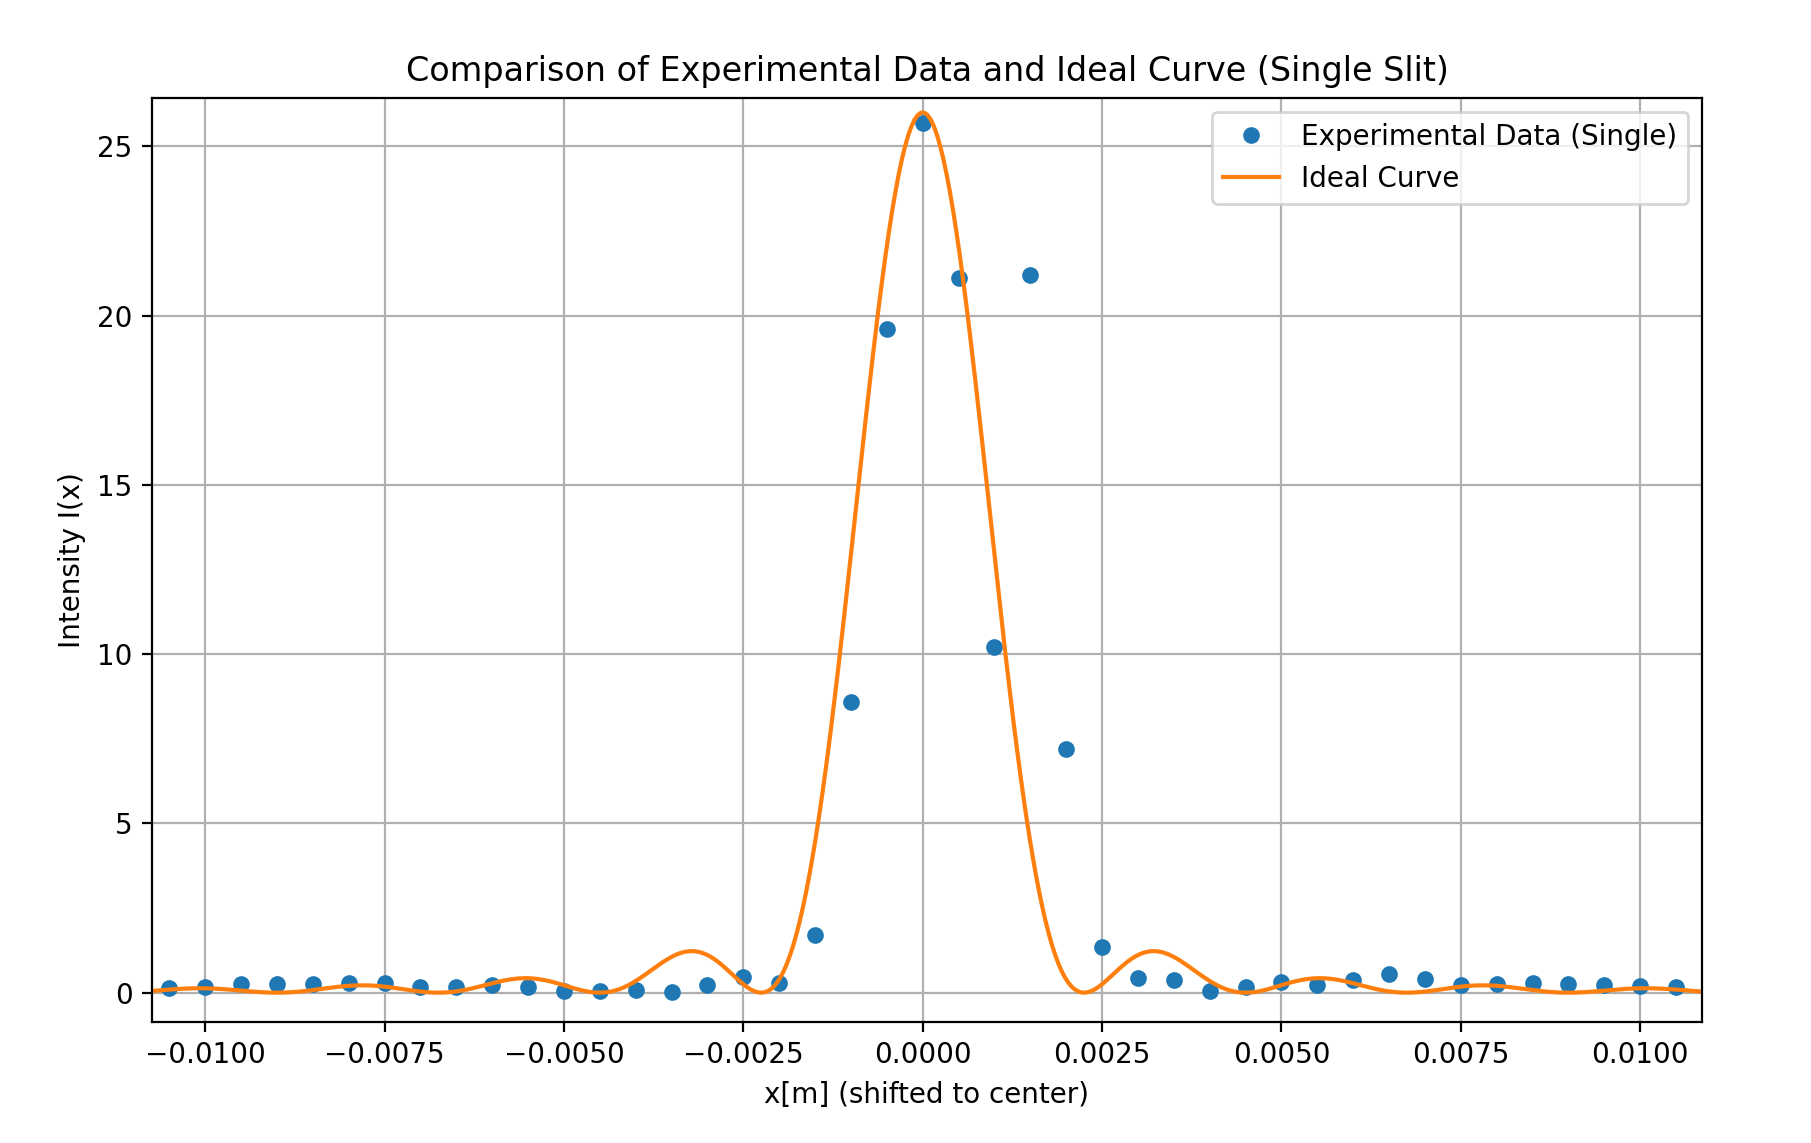
\includegraphics[width=100mm]{tan.png}
    \end{center}
    \caption{単スリットの強度分布の測定結果と理想曲線}
    \label{fig:tan}
\end{figure}

\subsection{複スリット}
複スリットのスリット幅の測定結果は、$a_{1} = 8.0 \times 10^{-5} \si{\meter}$、$a_{2} = 9.2 \times 10^{-5} \si{\meter}$であった。また、スリット間隔$d$は、$d_{\text{left}} = 8.1 \times 10^{-4} \si{ \meter} \quad d_{\text{right}}= 8.8 \times 10^{-4}\si{\meter}$であった。また、本実験では、スリットとスクリーンの距離$L$は、$L=30.0 \si{cm}$であった。
このもとで、測定結果と理想曲線は以下のようになった。
\begin{figure}[H]
    \begin{center}
    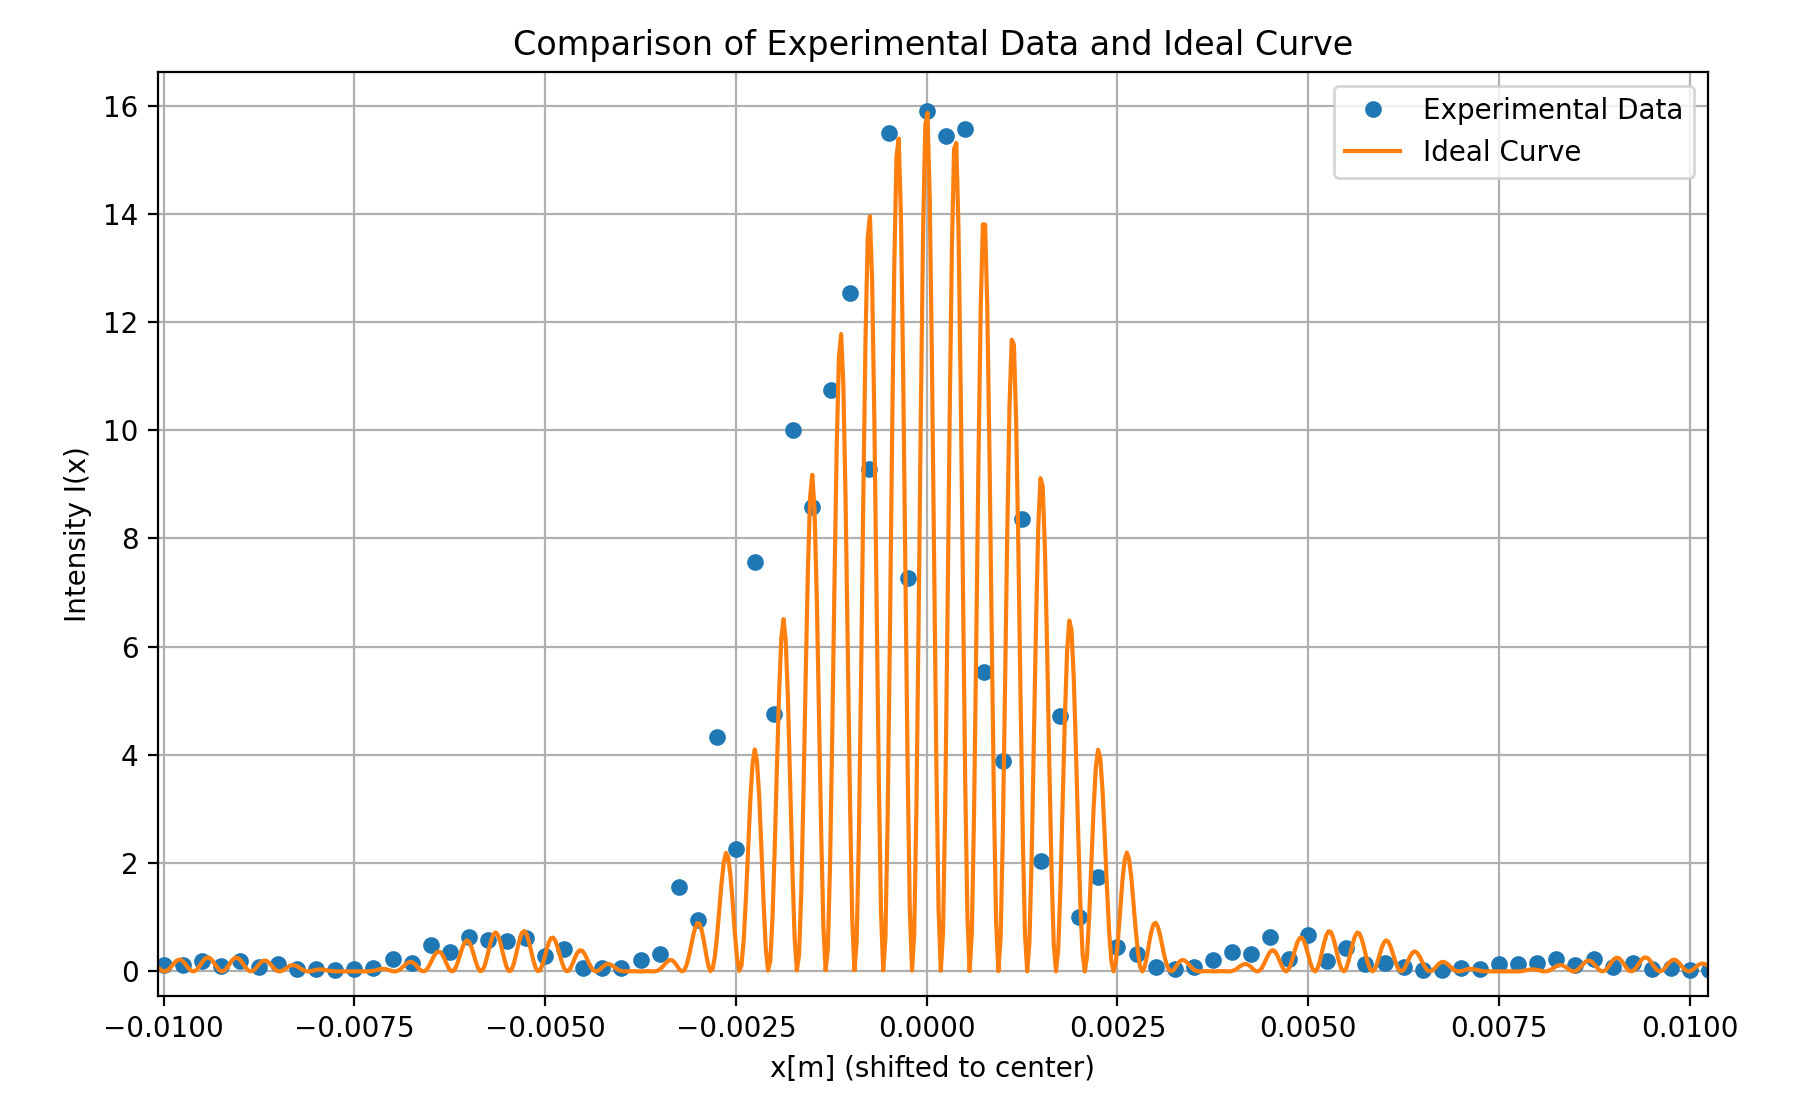
\includegraphics[width=100mm]{huku.png}
    \end{center}
    \caption{複スリットの強度分布の測定結果と理想曲線}
    \label{fig:huku1}
\end{figure}
ただし、平均をとって、スリット幅は$8.6 \times 10^{-5}\si{\meter}$とし、スリット間隔は$8.45\times 10^{-4}\si{\meter}$とした。
%推敲済

\subsection{分光シート}
\subsection{1つ目の分光シート}
スクリーンには、正方格子の干渉パターンが観測された。とくに、中心から横に離れた位置について、強め合う点同士の間隔は以下の表のようになった。(5箇所で測定した。)
\begin{table}[H]
  \centering
  \begin{tabular}{| c | c |}
    \hline
    \textbf{位置} & \textbf{強め合う点同士の間隔} \rule[-5mm]{0mm}{15mm} \\
    \hline
    1 & 0.0090 \si{\meter} \\
    2 & 0.0095 \si{\meter} \\
    3 & 0.0088 \si{\meter} \\
    4 & 0.0091 \si{\meter} \\
    5 & 0.0091 \si{\meter} \\
    \hline
  \end{tabular}
\end{table}
これらの平均をとって、スクリーン上での強め合う点同士の間隔は、$D = 0.0091 \si{\meter}$であった。また、スリットとスクリーンの距離$L$は、$L=10.0 \si{cm}$であった。\\
\textbf{格子の決定}\\
まず、格子間隔を決定することを考える。
原理の式から、格子間隔を$d$とすると、
\begin{align}
  \frac{2\pi}{d} = \frac{2\pi D}{\lambda L}
\end{align}
となる。ただし、$L$はシートとスクリーンとの距離。これを用いて格子間隔を求めると、
\begin{align}
  &\frac{1}{6.7 \times 10^{-7}} \times \frac{0.0091}{0.1} = \frac{1}{d}\\
   &d = 7.4 \times 10^{-6} \si{\meter}
\end{align}
となる。したがって、格子間隔は$7.4 \times 10^{-6} \si{\meter}$である。

また、逆格子は正方格子であったから、逆格子についても同様の形となることがわかる。したがって、今回用いた分光シートは、格子間隔が$7.4 \times 10^{-6} \si{\meter}$の正方格子であることがわかる。

\subsection{2つ目の分光シート}
測定の便宜上、シートを45度傾けて測定を行った。
スクリーンには、正方格子の干渉パターンが観測された。とくに、中心から横に離れた位置について、強め合う点同士の間隔は以下の表のようになった。(5箇所で測定した。)
\begin{table}[H]
  \centering
  \begin{tabular}{| c | c |}
    \hline
    \textbf{位置} & \textbf{強め合う点同士の間隔} \rule[-5mm]{0mm}{15mm} \\
    \hline
    1 & 0.0035 \si{\meter} \\
    2 & 0.00227 \si{\meter} \\
    3 & 0.00285 \si{\meter} \\
    4 & 0.00215 \si{\meter} \\
    5 & 0.0033 \si{\meter} \\
    \hline
  \end{tabular}
\end{table}
これらの平均をとって、スクリーン上での強め合う点同士の間隔は、$D = 0.002814 \si{\meter}$であった。また、スリットとスクリーンの距離$L$は、$L=10.0 \si{cm}$であった。\\
\textbf{格子の決定}\\
まず、格子間隔を決定することを考える。
原理の式から、格子間隔を$d$とすると、
\begin{align}
  \frac{2\pi}{d} = \frac{2\pi D}{\lambda L}
\end{align}
となる。ただし、$L$はシートとスクリーンとの距離。これを用いて格子間隔を求めると、
\begin{align}
  &\frac{1}{6.7 \times 10^{-7}} \times \frac{0.002814}{0.1} = \frac{1}{d}\\
   &d = 2.3 \times 10^{-5} \si{\meter}
\end{align}
となる。したがって、格子間隔は$2.3 \times 10^{-5} \si{\meter}$である。

また、逆格子は正方格子であったから、逆格子についても同様の形となることがわかる。したがって、今回用いた分光シートは、格子間隔が$7.4 \times 10^{-6} \si{\meter}$の正方格子を、45度傾けて用いたものであることがわかる。
%推敲済

\section{考察}
\subsection{単スリット}
\subsubsection{ピークまわりについて}
単スリットの測定結果について、ピーク付近におけるドットが、右側だけいくらか理想曲線からずれていることがわかる。これは、測定時に、中心から左方向を測定したのち、中央に戻って、その後右方向を測定したため、その最中に台がずれてしまうなどしたことが原因だと考えられる。\\

\subsection{複スリット}
\subsubsection{ピークまわりについて}
複スリットの測定結果について、ピーク付近におけるドットが、理想曲線に沿ってはいるものの、完全に追跡できてはいないこともわかる。
これは、ピーク付近での強度変化が非常に急激であるため、この測定の粗さでは追跡しきれていないことを表している。さらに正確なデータを得るためには、一回あたりに動かす距離を小さくすると良いことがわかる。
具体的には、一回当たりの長さを以下のように見積もればよい。

\begin{align}
  d\sin\theta = n\lambda
\end{align}
について、$\sin\theta = \frac{x}{L}$であるから、
\begin{align}
  x = \frac{n\lambda L}{d}
\end{align}
となる。これに数値を代入することで、
\begin{align}
  \delta x = \frac{1 \times 6.7 \times 10^{-7} \si{\meter}}{8.1 \times 10^{-4}\si{\meter}} \times 0.3\si{\meter} = 2.48 \times 10^{-3} \si{\meter}
\end{align}
となる。したがって、この値よりも小さくすることで、より正確なデータを得ることができると考えられる。

\subsubsection{左右差について}
実際には、各スリットの幅が異なるため、その分プロットと理想曲線との間にずれが生じてしまうと考えらえる。したがって、このずれを考慮するためには、理想曲線を修正する必要がある。\\
\textbf{修正方法}\\
スリット1およびスリット2からの電場は、それぞれ次のように表される
\begin{align}
    E_1(x) &= A_1 \mathrm{sinc} \left( \frac{\pi a_1 x}{\lambda L} \right) \\
    E_2(x) &= A_2 \mathrm{sinc} \left( \frac{\pi a_2 x}{\lambda L} \right) e^{i \Delta \phi}
\end{align}
ここで、\(\mathrm{sinc}(u) = \frac{\sin(u)}{u}\) は単スリット回折の因子を表し、\(\Delta \phi\) はスリット間による位相差であり次式で与えられる。
\begin{align}
    \Delta \phi = \frac{2\pi d x}{\lambda L}.
\end{align}
スリットでの合成電場 \(E(x)\) は、スリット1およびスリット2からの電場の重ね合わせとして次のように表される。
\begin{align}
    E(x) = A_1 \mathrm{sinc} \left( \frac{\pi a_1 x}{\lambda L} \right) + A_2 \mathrm{sinc} \left( \frac{\pi a_2 x}{\lambda L} \right) e^{i \Delta \phi}.
\end{align}
このとき、
光の強度 \(I(x)\) は電場の絶対値の二乗として定義される
\begin{align}
    I(x) = |E(x)|^2
\end{align}
すなわち、
\begin{align}
    I(x) &= \left| A_1 \mathrm{sinc} \left( \frac{\pi a_1 x}{\lambda L} \right) + A_2 \mathrm{sinc} \left( \frac{\pi a_2 x}{\lambda L} \right) e^{i \Delta \phi} \right|^2
\end{align}
となる。

これをもとに、左右差をもたせて強度分布をプロットすると、以下のようになる。
\begin{figure}[H]
    \begin{center}
    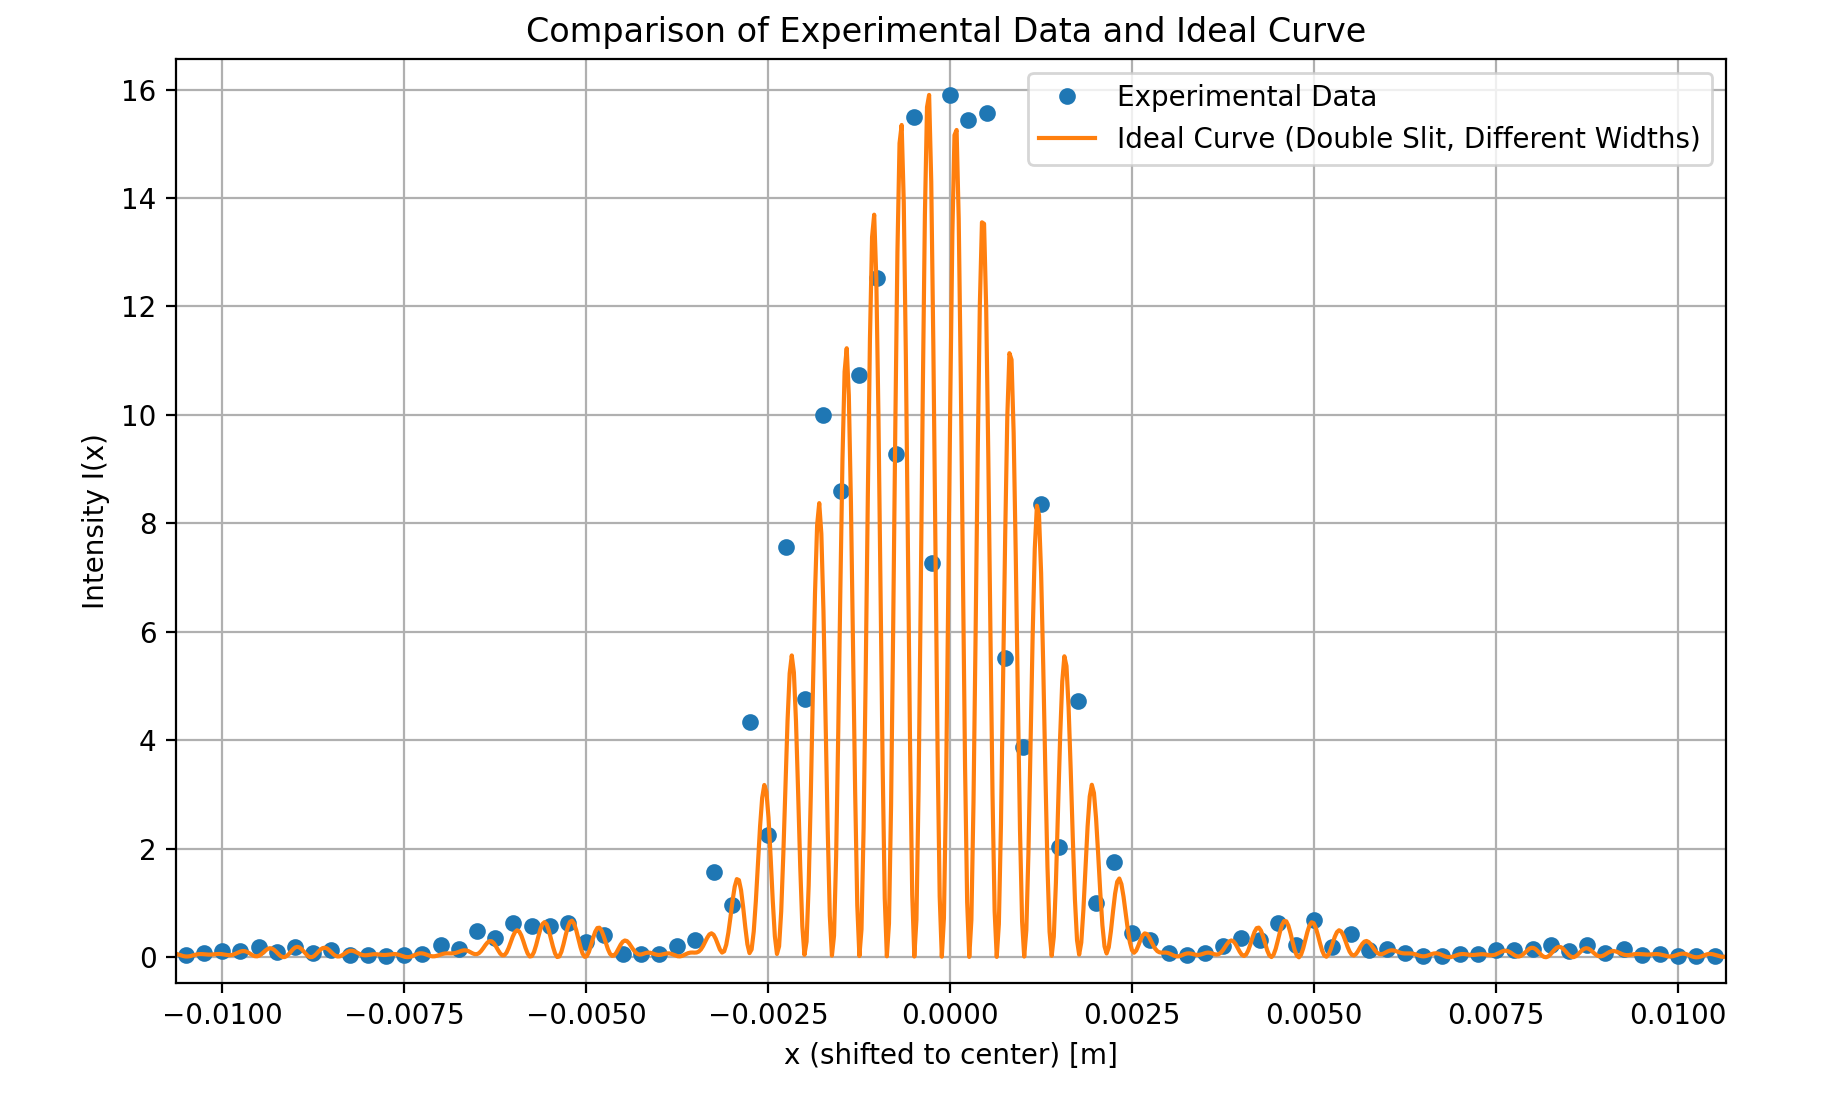
\includegraphics[width=100mm]{huku2.png}
    \end{center}
    \caption{複スリットの強度分布の測定結果と理想曲線(左右差あり)}
    \label{fig:huku2}
\end{figure}
これを見ると、左右差をもたせていないときに比べて、ピークの部分の裾が狭まっていることがわかる。これは、実験データに対して以前よりもよくフィットしていることを示している。


\subsection{X線実験との関連性}
X線回折との関連性をみる。X線回折の理論について以下にまとめる。
\subsubsection{X線回折の理論}
結晶中の原子配置を密度関数 \(\rho(\bm{r})\) で表す。この密度関数は、結晶中の周期的な原子配置を反映して次のように書ける。
\begin{align}
    \rho(\bm{r}) = \sum_{\bm{R}} f(\bm{r} - \bm{R})
\end{align}
ここで、
\begin{itemize}
    \item \(\bm{R}\):格子点の位置ベクトル。
    \item \(f(\bm{r})\):単位格子内の原子配置を表す密度分布。
\end{itemize}
である。

X線が結晶に入射したとき、結晶内の各点から散乱される波が干渉する。このとき、散乱波の振幅 \(A(\bm{q})\) は次のように記述される。
\begin{align}
    A(\bm{q}) = \int \rho(\bm{r}) e^{i \bm{q} \cdot \bm{r}} \, d\bm{r}
\end{align}
ただし、
\begin{itemize}
    \item \(\bm{q} = \bm{k}_{\text{out}} - \bm{k}_{\text{in}}\):散乱ベクトル
    \item \(\bm{k}_{\text{in}}, \bm{k}_{\text{out}}\):それぞれ入射波と散乱波の波数ベクトル
\end{itemize}
この式は、密度関数 \(\rho(\bm{r})\) のフーリエ変換を表している。

\(\rho(\bm{r})\) を上の周期的なモデルに代入すると、振幅 \(A(\bm{q})\) は次のように書ける。
\begin{align}
    A(\bm{q}) &= \int \sum_{\bm{R}} f(\bm{r} - \bm{R}) e^{i \bm{q} \cdot \bm{r}} \, d\bm{r}\\
     &= \sum_{\bm{R}} e^{i \bm{q} \cdot \bm{R}} \int f(\bm{r}) e^{i \bm{q} \cdot \bm{r}} \, d\bm{r}
\end{align}
ここで、
\begin{itemize}
    \item \(\sum_{\bm{R}} e^{i \bm{q} \cdot \bm{R}}\):結晶格子の周期性に起因する項(逆格子ベクトル \(\bm{G}\) にピークを生じさせる)
    \item \(\int f(\bm{r}) e^{i \bm{q} \cdot \bm{r}} \, d\bm{r}\):単位格子内の原子配置のフーリエ変換
\end{itemize}

単位格子内の原子配置に依存する部分を\textbf{構造因子} \(F(\bm{G})\) として定義すると、
\begin{align}
    F(\bm{G}) = \sum_j f_j e^{i \bm{G} \cdot \bm{r}_j},
\end{align}
ここで、
\begin{itemize}
    \item \(f_j\):単位格子内の原子 \(j\) の散乱因子。
    \item \(\bm{r}_j\):単位格子内の原子 \(j\) の位置。
    \item \(\bm{G}\):逆格子ベクトル。
\end{itemize}

これにより、振幅 \(A(\bm{q})\) は次のように書ける。
\begin{align}
    A(\bm{q}) = \sum_{\bm{G}} F(\bm{G}) \delta(\bm{q} - \bm{G})
\end{align}

\(\bm{q}\) が逆格子ベクトル \(\bm{G}\) に一致する場合にのみ、振幅 \(A(\bm{q})\) は非ゼロとなる。この条件は、ブラッグ条件
\begin{align}
    2d \sin\theta = n\lambda
\end{align}
に対応する。

回折パターンで観測される強度 \(I(\bm{q})\) は、振幅の絶対値の2乗として与えられる。
\begin{align}
    I(\bm{q}) \propto \left| F(\bm{G}) \right|^2
\end{align}

フーリエ変換を用いて、以下の関係が成立する。
\begin{align}
    \rho(\bm{r}) \xrightarrow{\text{フーリエ変換}} A(\bm{q}) \xrightarrow{\text{逆フーリエ変換}} \rho(\bm{r})
\end{align}

これにより、回折パターン(逆空間データ)から実空間の結晶構造を再構築できる。

\subsubsection{分光シートとの関連性}
原理の分光シートについての記述と、上でのX線回折の理論との関連性を考える。X線回折における結晶の原子配置と、分光シートにおける格子の関係性を考えると、分光シートはX線回折の理論と非常に類似していることがわかる。したがって、分光シートを用いることで、X線回折の理論を直接観測することができると考えられる。
\begin{align}
  \rho(\bm{r}) = \sum_{\bm{R}} f(\bm{r} - \bm{R}) \leftrightarrow A(x) = \sum_{n=-\infty}^\infty \delta(x - n d)
\end{align}
となっていることがわかる。さらに、それぞれフーリエ変換を行うと、
\begin{align}
  A(\bm{q}) = \sum_{\bm{G}} F(\bm{G}) \delta(\bm{q} - \bm{G}) \leftrightarrow E(k_x) = \frac{1}{d} \sum_{m=-\infty}^\infty \delta\left(k_x - \frac{2\pi m}{d}\right)
\end{align}
となる。したがって、分光シートを通してシートの構造の逆格子が得られることに対応して、X線回折の理論においても、逆格子ベクトルに対応するピークが得られることがわかる。





\begin{thebibliography}{99}
  \bibitem{ref} 北海道大学理学部物理学科, 『物理学実験』, 2024 ,p53-72
\end{thebibliography}

\end{document}